%\documentclass[aspectratio=169]
\documentclass[aspectratio=169,xcolor=dvipsnames]{beamer}
%\usetheme{Copenhagen}
\usetheme{boxes}
\setbeamertemplate{navigation symbols}{}
\setbeamertemplate{footline}[frame number]
%\setbeamertemplate{footline}{}
\usecolortheme{dove}   %[named=black]
\usepackage{appendixnumberbeamer}
\usepackage[utf8]{inputenc}

\usepackage{graphicx}         
\graphicspath{ {./Pictures/} }
\usepackage{amsmath}
\usepackage{amsfonts}
\usepackage{amssymb}
\usepackage{amsthm}
\usepackage{mathtools}
\usepackage{commath}
\usepackage{multimedia}
\usepackage{multirow}
\usepackage{subcaption}
\usepackage{numprint032}
\usepackage[style=verbose,backend=bibtex]{biblatex}
\addbibresource{PresentationBib.bib}
\usepackage{media9}
\addmediapath{Animations/}
\newcommand{\Sta}{y}
\newcommand{\Adj}{p}
\newcommand{\Con}{u}


\begin{document}

\title[]{Numerical Methods for PDE-Constrained Optimization of Particle Dynamics}
\author[Jonna Roden]{Jonna Roden}
\institute[UoE]{University of Edinburgh/MIGSAA\\ 
	\vspace{0.2cm}
	Joint work with Ben Goddard and John Pearson}
\date{12th July 2021}

\begin{frame}
\titlepage
\end{frame}
 
 
\begin{frame}
	\frametitle{Structure of the Talk}
	 
	 \begin{itemize}
	 	\item The Optimization Problem
	 	\item Numerical Methods\\
	 	\begin{itemize}
	 		\item Pseudospectral and Spectral Element Methods
	 		\item Fixed Point Algorithm
	 		\item Newton-Krylov Algorithm
	 	\end{itemize}
	 	\item Results
	 \end{itemize}
\end{frame}

\begin{frame}
	\frametitle{The Optimization Problem}
%	\begin{columns}


%		\column{0.8 \linewidth}
		\begin{align*}
		&\min_{\rho,\vec{w}} \quad \frac{1}{2}\norm{\rho- \widehat{\rho}}_{L_2(\Sigma)}^2 + \frac{\beta}{2} \norm{\vec{w}}_{L_2(\Sigma)}^2\\
		\\
		&\text{subject to:}
		\\
		& \partial_t \rho = \nabla^2 \rho - \nabla \cdot (\rho \vec{w}) + \nabla \cdot \left(\rho \nabla V_{ext}\right)+\nabla \cdot \int_\Omega \rho(\vec{x}) \rho(\vec{x}\hspace{0.2em}') \nabla V_2(|\vec{x}-\vec{x}\hspace{0.2em}'|)d\vec{x}\hspace{0.2em}' \qquad { \text{in    } \Sigma}\\
		\\
		&{\text{BC } \text{and IC:}}\\
		&\frac{\partial \rho}{\partial n} - \rho \vec{w} \cdot \vec{n} + \rho \frac{\partial V_{ext}}{\partial n} +   \int_\Omega \rho(\vec{x}) \rho(\vec{x}\hspace{0.2em}')  \frac{ \partial  V_2}{\partial n}(|\vec{x}-\vec{x}\hspace{0.2em}'|)d\vec{x}\hspace{0.2em}'= 0 \quad \ \ \qquad \qquad \qquad \quad \text{on   } \partial \Sigma   \\
		&{\rho(0,\vec{x}) = \rho_0(\vec{x})} 
		\end{align*}
%		\column{0.2 \linewidth}
%		\vspace{-1cm}
%		\begin{figure}	
%			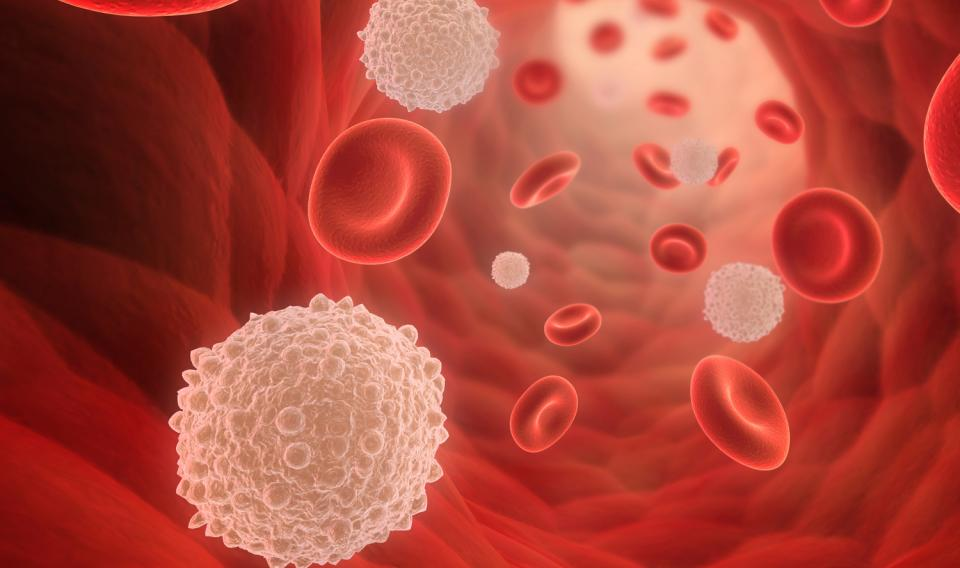
\includegraphics[width=3cm]{bloodcells.jpg}\\
%			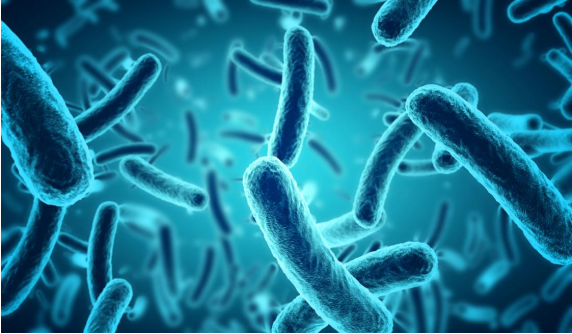
\includegraphics[width=3cm]{bacteria.png}\\			
%			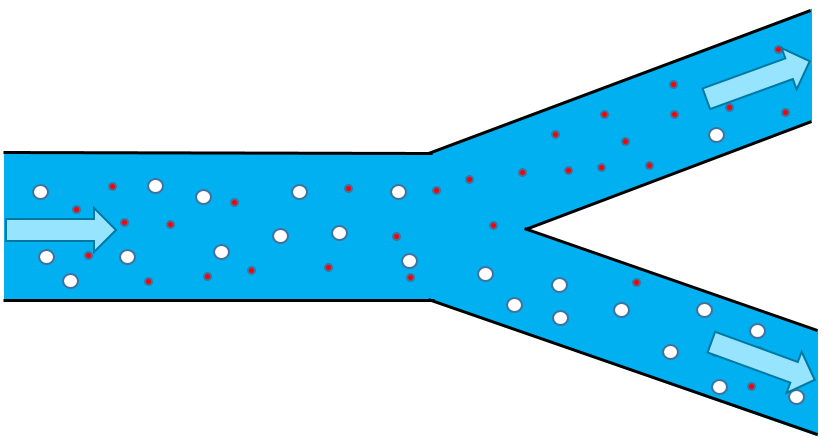
\includegraphics[width=3cm]{Microfilter.png}\\
%			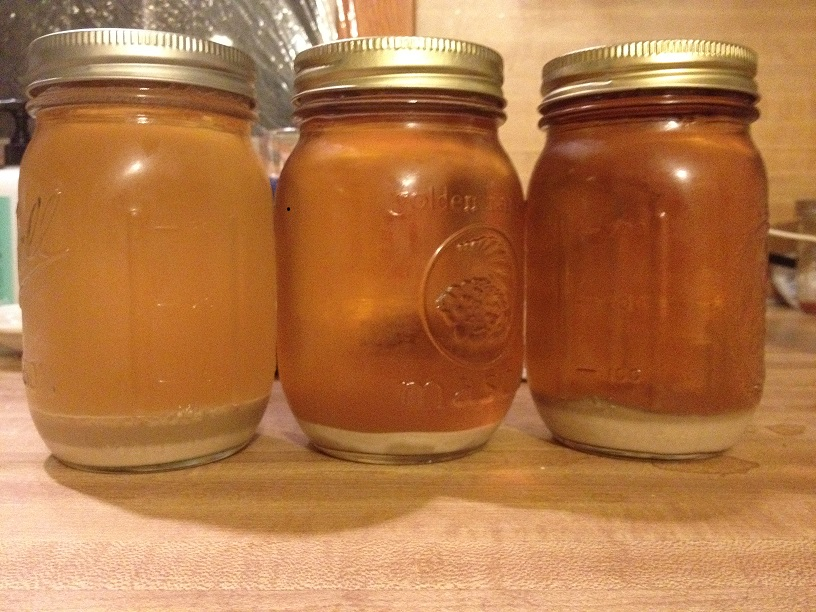
\includegraphics[width=3cm]{beer.png}
%		\end{figure}
%	\end{columns}
\end{frame}

\begin{frame}
	\frametitle{The Optimization Problem}
	\textbf{The (first-order) optimality system}\\
     
	\begin{align*}
	 \partial_t \rho &= \nabla^2 \rho - \nabla \cdot (\rho \textcolor{blue}{\vec{w}}) + \nabla \cdot \left(\rho \nabla V_{ext}\right)
	+ \nabla \cdot \int_\Omega \rho(\vec{x}) \rho(\vec{x}\hspace{0.2em}') \nabla V_2(|\vec{x}-\vec{x}\hspace{0.2em}'|)d\vec{x}\hspace{0.2em}'  \\
	\partial_t q &= -\nabla^2 q - \nabla q \cdot \textcolor{blue}{\vec{w}} + \nabla q \cdot \nabla V_{ext} + \int_\Omega \textcolor{ForestGreen}{\rho(\vec{x}\hspace{0.2em}')} \bigg(\nabla q(\vec{x}) + \nabla q(\vec{x}\hspace{0.2em}')\bigg)\cdot  \nabla V_2(|\vec{x}-\vec{x}\hspace{0.2em}'|)d\vec{x}\hspace{0.2em}' \\
    \textcolor{blue}{\vec{w}} \ &= - \frac{1}{\beta}\textcolor{ForestGreen}{\rho} \nabla  \textcolor{red}{q}\\
    \\
    \rho(0,\vec{x})&=\rho_0(\vec{x}), \qquad q(T,\vec{x})= 0, \qquad \qquad \text{+BCs}\\
	\end{align*}
\end{frame}




\begin{frame}
	\frametitle{Numerical Methods}

	\begin{itemize} 
		\item Challenge 1: Particle interaction term is nonlinear and nonlocal (+ nonlocal BCs).
		\\How to avoid shortcomings of standard methods (FEM/FDM)?\\
		\vspace{0.3 cm}		
		\textbf{$\Rightarrow$ Pseudospectral Method}\\
		\ \ \ \ AND\\
		\textbf{$\Rightarrow$ Spectral Element Method}		
		\vspace{0.2 cm}
		\item Challenge 2: One PDE has an initial, the other a final time condition. The Laplacians have opposite signs. \\How to do time stepping?\\
		\vspace{0.3 cm}	
		\textbf{$\Rightarrow$ Fixed Point Algorithm}\\
		\ \ \ \ OR\\
		\textbf{$\Rightarrow$ Newton-Krylov Algorithm}
	\end{itemize}

\end{frame}


\begin{frame}
	\frametitle{Pseudospectral Method}
\begin{figure}
	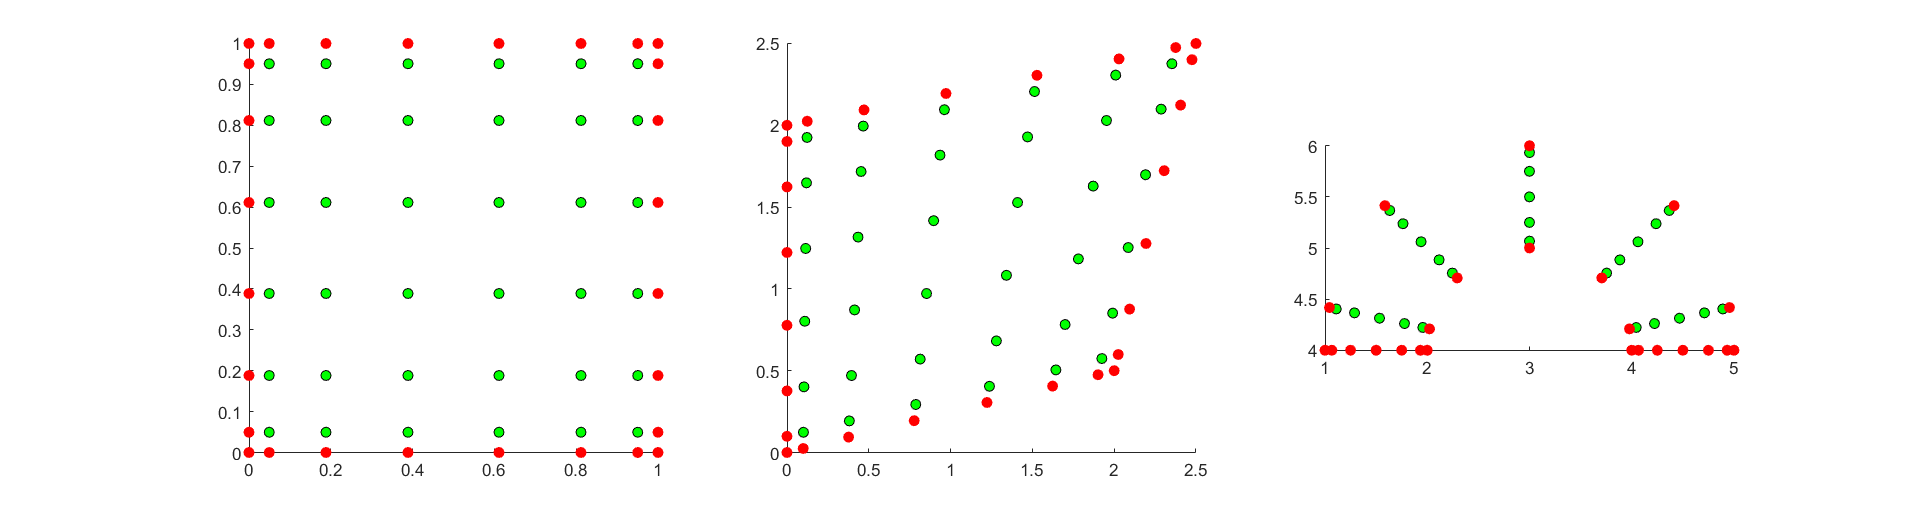
\includegraphics[width=15cm]{Shapes1.png}
\end{figure}
    \begin{itemize}
    	\item Reduce both PDEs to systems of ODEs.
    	\item Discretize time (accurate interpolation).
    	\item Equations can now be solved using the Fixed Point Algorithm (with DAE solvers) or the Newton-Krylov Algorithm.
    \end{itemize}
	
\end{frame}
\begin{frame}
	\frametitle{Spectral Element Method}
	\begin{figure}
		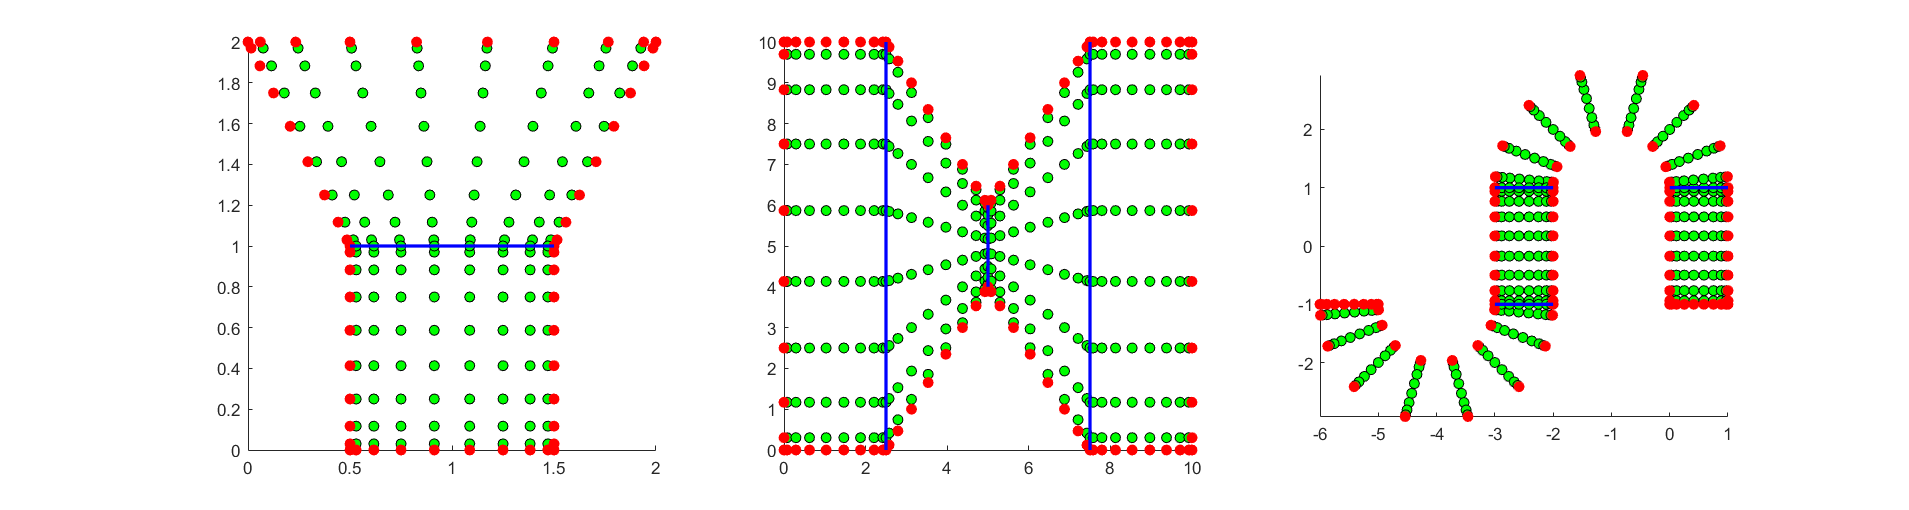
\includegraphics[width=15cm]{MultiShapes.png}
	\end{figure}
		\begin{itemize}
			\item Discretize PDE on each element using pseudospectral methods.
			\item Match solution and flux between elements.
		\end{itemize}
		

	
	
\end{frame}
\begin{frame}
	\frametitle{Fixed Point Algorithm}
	\textbf{The (first-order) optimality system}\\
	
	\begin{align*}
		\partial_t \rho &= \nabla^2 \rho - \nabla \cdot (\rho \textcolor{blue}{\vec{w}}) + \nabla \cdot \left(\rho \nabla V_{ext}\right)
		+ \nabla \cdot \int_\Omega \rho(\vec{x}) \rho(\vec{x}\hspace{0.2em}') \nabla V_2(|\vec{x}-\vec{x}\hspace{0.2em}'|)d\vec{x}\hspace{0.2em}'  \\
		\partial_t q &= -\nabla^2 q - \nabla q \cdot \textcolor{blue}{\vec{w}} + \nabla q \cdot \nabla V_{ext} + \int_\Omega \textcolor{ForestGreen}{\rho(\vec{x}\hspace{0.2em}')} \bigg(\nabla q(\vec{x}) + \nabla q(\vec{x}\hspace{0.2em}')\bigg)\cdot  \nabla V_2(|\vec{x}-\vec{x}\hspace{0.2em}'|)d\vec{x}\hspace{0.2em}' \\
		\textcolor{blue}{\vec{w}} \ &= - \frac{1}{\beta}\textcolor{ForestGreen}{\rho} \nabla  \textcolor{red}{q}\\
		\\
		\rho(0,\vec{x})&=\rho_0(\vec{x}), \qquad q(T,\vec{x})= 0, \qquad \qquad \text{+BCs}\\
	\end{align*}
\end{frame}

\begin{frame}
	\frametitle{Fixed Point Algorithm}

Initialize with guess $\textcolor{blue}{\vec{w}^{(0)}}$.
	\begin{enumerate}
     \item 
     Solve $\displaystyle \partial_t \rho  = \nabla^2 \rho  - \nabla \cdot (\rho \textcolor{blue}{\vec{w}^{(i)}} ) + \nabla \cdot \left(\rho \nabla V_{ext}\right)
     + \nabla \cdot \int_\Omega \rho(\vec{x}) \rho(\vec{x}\hspace{0.2em}') \nabla V_2(|\vec{x}-\vec{x}\hspace{0.2em}'|)d\vec{x}\hspace{0.2em}'. 
     $
	 \item
     Solve $\displaystyle \partial_{{\tau}} q  = \nabla^2 q  + \nabla q  \cdot \textcolor{blue}{\vec{w}^{(i)}}  - \nabla q \cdot \nabla V_{ext}$\\
     $\qquad \qquad \quad \ \ \displaystyle - \int_\Omega \textcolor{ForestGreen}{\rho^{(i)}(\vec{x}\hspace{0.2em}')} \bigg(\nabla q( \vec{x} ) + \nabla q( \vec{x}\hspace{0.2em}')\bigg) \cdot \nabla V_2(|\vec{x}-\vec{x}\hspace{0.2em}'|)d\vec{x}\hspace{0.2em}'. 
     $
     \item Solve $\displaystyle \textcolor{blue}{\vec{w}^{(i)}_g} = - \frac{1}{\beta}\textcolor{ForestGreen}{{\rho}^{(i)}} \nabla \textcolor{red}{{q}^{(i)}}.$
     \vspace{0.4 cm}
     \item Measure the error: $ \mathcal{E} = ||\textcolor{blue}{\vec{w}^{(i)}} - \textcolor{blue}{\vec{w}^{(i)}_g}||$.
     \vspace{0.2 cm}
	 \item Update control, with $\lambda \in [0,1]$:       $\quad \textcolor{blue}{\vec{w}^{(i+1)}} = (1-\lambda)\textcolor{blue}{\vec{w}^{(i)}} + \lambda \textcolor{blue}{\vec{w}^{(i)}_g}.$	 
	\end{enumerate}	
\vspace{0.2 cm}
Iterate until $\mathcal{E} <TOL$.
\end{frame}
\begin{frame}
	\frametitle{Reminder: The Optimization Problem}
	%	\begin{columns}
	
	
	%		\column{0.8 \linewidth}
	\begin{align*}
		&\min_{\rho,\vec{w}} \quad \frac{1}{2}\norm{\rho- \widehat{\rho}}_{L_2(\Sigma)}^2 + \frac{\beta}{2} \norm{\vec{w}}_{L_2(\Sigma)}^2\\
		\\
		&\text{subject to:}
		\\
		& \partial_t \rho = \nabla^2 \rho - \nabla \cdot (\rho \vec{w}) + \nabla \cdot \left(\rho \nabla V_{ext}\right)+\nabla \cdot \int_\Omega \rho(\vec{x}) \rho(\vec{x}\hspace{0.2em}') \nabla V_2(|\vec{x}-\vec{x}\hspace{0.2em}'|)d\vec{x}\hspace{0.2em}' \qquad { \text{in    } \Sigma}\\
		\\
		&{\text{BC } \text{and IC:}}\\
		&\frac{\partial \rho}{\partial n} - \rho \vec{w} \cdot \vec{n} + 	\rho \frac{\partial V_{ext}}{\partial n} +   \int_\Omega \rho(\vec{x}) \rho(\vec{x}\hspace{0.2em}')  \frac{ \partial  V_2}{\partial n}(|\vec{x}-\vec{x}\hspace{0.2em}'|)d\vec{x}\hspace{0.2em}'= 0 \quad \ \ \qquad \qquad \qquad \quad \text{on   } \partial \Sigma   \\
		&{\rho(0,\vec{x}) = \rho_0(\vec{x})} 
	\end{align*}
	%		\column{0.2 \linewidth}
	%		\vspace{-1cm}
	%		\begin{figure}	
	%			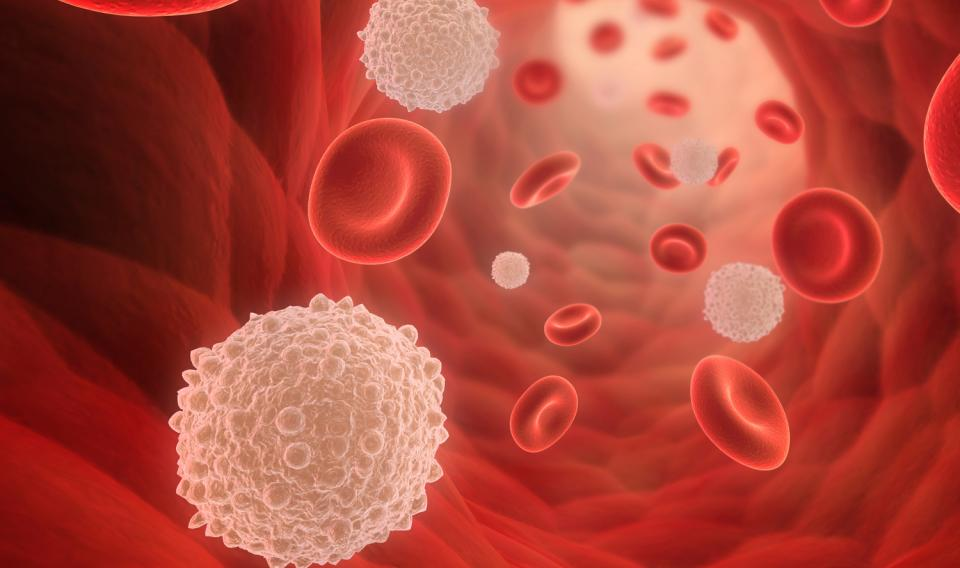
\includegraphics[width=3cm]{bloodcells.jpg}\\
	%			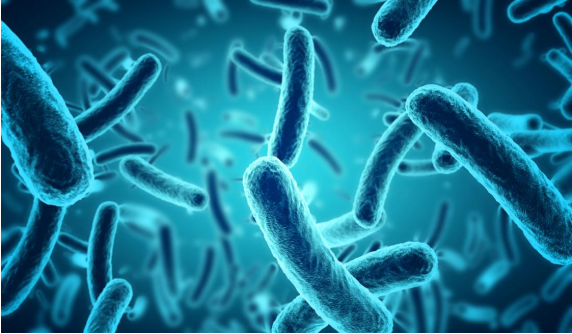
\includegraphics[width=3cm]{bacteria.png}\\			
	%			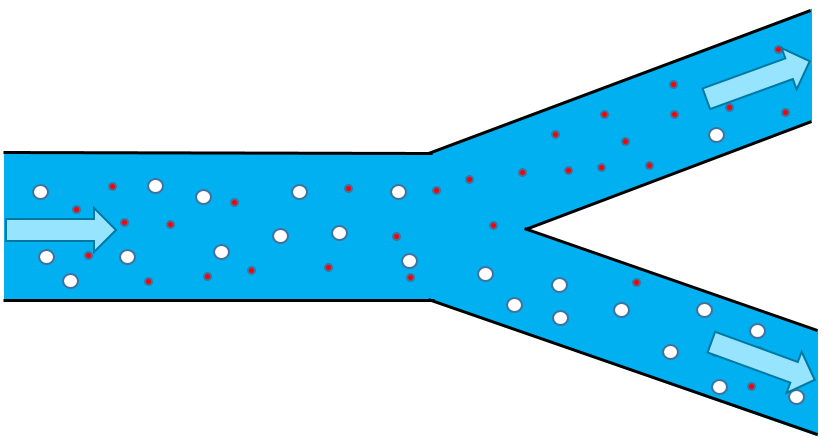
\includegraphics[width=3cm]{Microfilter.png}\\
	%			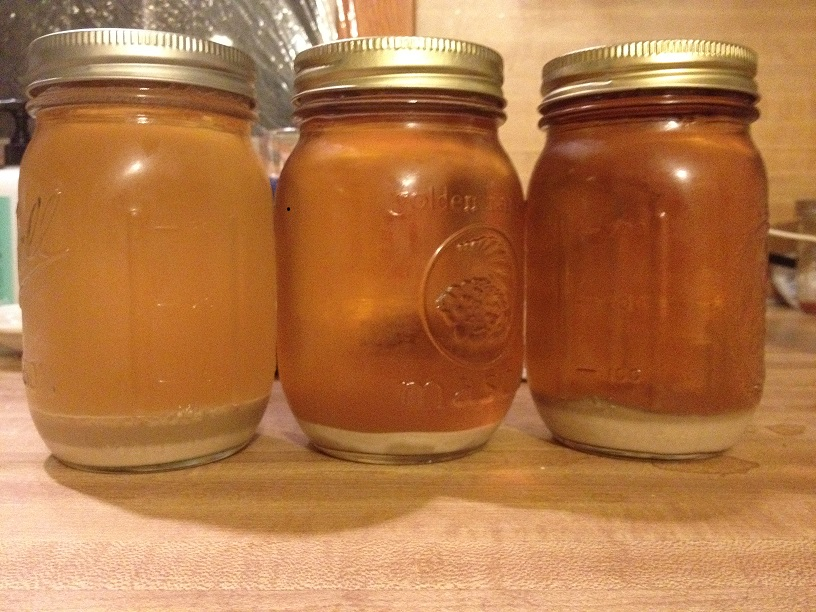
\includegraphics[width=3cm]{beer.png}
	%		\end{figure}
	%	\end{columns}
\end{frame}

\begin{frame}
	\frametitle{Fixed Point Algorithm Results}
	Overall Cost: $\mathcal J = \frac{1}{2}\norm{\rho- \widehat{\rho}}_{L_2(\Sigma)}^2 + \frac{\beta}{2} \norm{\vec{w}}_{L_2(\Sigma)}^2$, $\mathcal J_{\vec{w}= \vec 0} = 0.0484$.
	\vspace{0.3 cm}
	\begin{figure}
		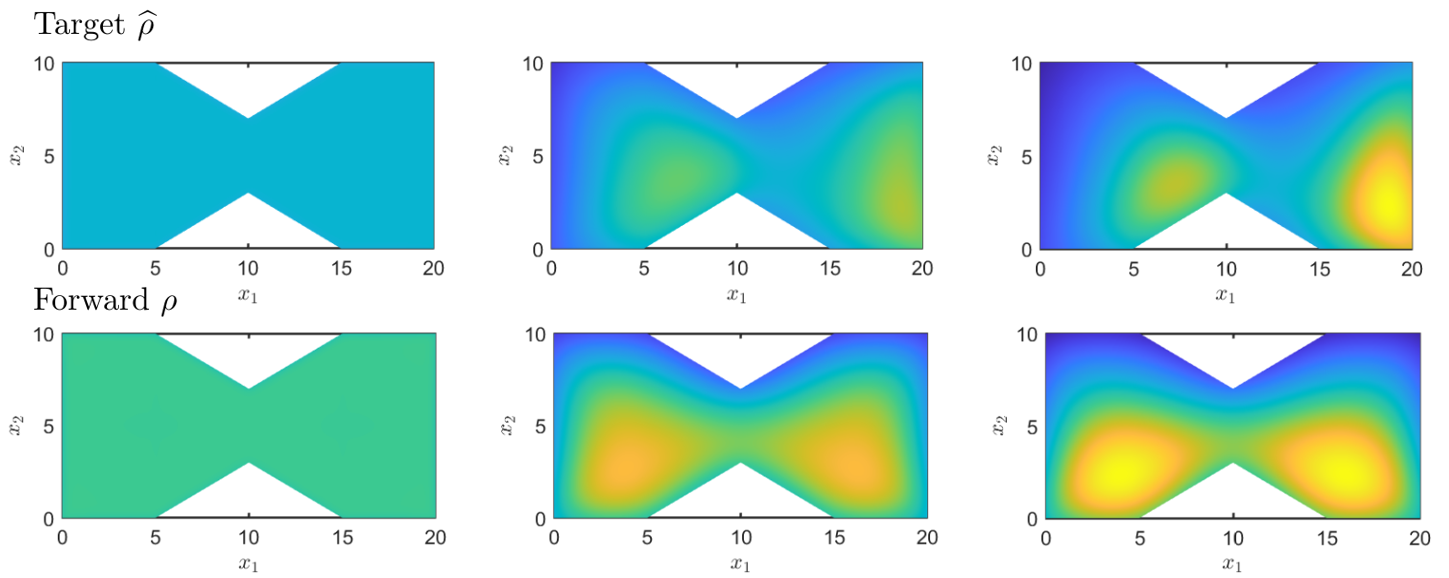
\includegraphics[width=14cm]{ExRes2a2.png}
	\end{figure}
	
\end{frame}
\begin{frame}
	\frametitle{Fixed Point Algorithm Results}
	\vspace{0.3cm}
	Overall Cost: $\mathcal J = \frac{1}{2}\norm{\rho- \widehat{\rho}}_{L_2(\Sigma)}^2 + \frac{\beta}{2} \norm{\vec{w}}_{L_2(\Sigma)}^2$, $\mathcal J_{\vec{w} = \vec 0} = 0.0484$, $\mathcal J_{\text{opt}} = 0.0146$.
	\begin{figure}
		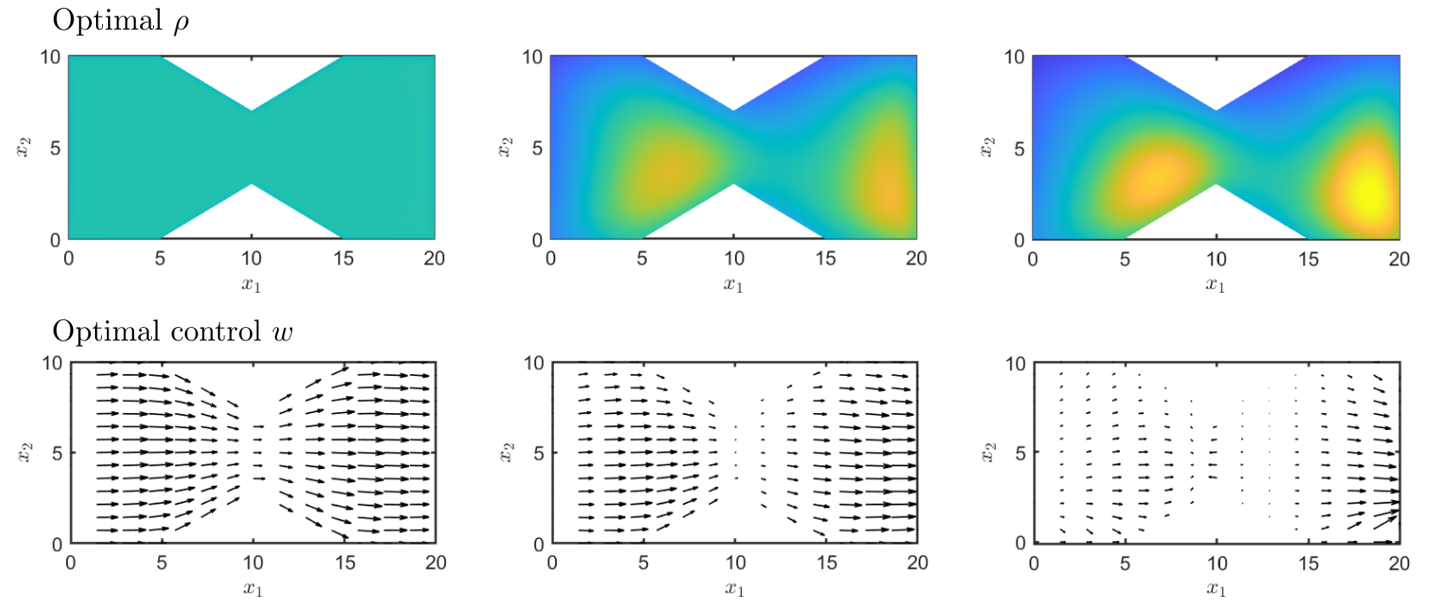
\includegraphics[width=14cm]{ExRes2b3.png}
	\end{figure}
\end{frame}

\begin{frame}
	\frametitle{Newton-Krylov Algorithm}
	\textbf{The (first-order) optimality system}\\
	\begin{align*}
		\partial_t \rho &= \nabla^2 \rho - \nabla \cdot (\rho \textcolor{blue}{\vec{w}}) + \nabla \cdot \left(\rho \nabla V_{ext}\right)
		+ \nabla \cdot \int_\Omega \rho(\vec{x}) \rho(\vec{x}\hspace{0.2em}') \nabla V_2(|\vec{x}-\vec{x}\hspace{0.2em}'|)d\vec{x}\hspace{0.2em}'  \\
		\partial_t q &= -\nabla^2 q - \nabla q \cdot \textcolor{blue}{\vec{w}} + \nabla q \cdot \nabla V_{ext} + \int_\Omega \textcolor{ForestGreen}{\rho(\vec{x}\hspace{0.2em}')} \bigg(\nabla q(\vec{x}) + \nabla q(\vec{x}\hspace{0.2em}')\bigg)\cdot  \nabla V_2(|\vec{x}-\vec{x}\hspace{0.2em}'|)d\vec{x}\hspace{0.2em}' \\
		\textcolor{blue}{\vec{w}} \ &= - \frac{1}{\beta}\textcolor{ForestGreen}{\rho} \nabla  \textcolor{red}{q}\\
		\\
		\rho(0,\vec{x})&=\rho_0(\vec{x}), \qquad q(T,\vec{x})= 0, \qquad \qquad \text{+BCs}\\
	\end{align*}
\end{frame}
\begin{frame}
	\frametitle{Newton-Krylov Algorithm}

	\begin{align*}
		\partial_t \rho &= \nabla^2 \rho + \frac{1}{\beta}\nabla \cdot (\rho  \textcolor{ForestGreen}{\rho} \nabla  \textcolor{red}{q}) + \nabla \cdot \left(\rho \nabla V_{ext}\right)
		+ \nabla \cdot \int_\Omega \rho(\vec{x}) \rho(\vec{x}\hspace{0.2em}') \nabla V_2(|\vec{x}-\vec{x}\hspace{0.2em}'|)d\vec{x}\hspace{0.2em}'  \\
		\partial_t q &= -\nabla^2 q + \frac{1}{\beta}\nabla q \cdot  \textcolor{ForestGreen}{\rho} \nabla  \textcolor{red}{q}  + \nabla q \cdot \nabla V_{ext} \\
		& \quad+ \int_\Omega \textcolor{ForestGreen}{\rho(\vec{x}\hspace{0.2em}')} \bigg(\nabla q(\vec{x}) + \nabla q(\vec{x}\hspace{0.2em}')\bigg)\cdot  \nabla V_2(|\vec{x}-\vec{x}\hspace{0.2em}'|)d\vec{x}\hspace{0.2em}' \\
		\\
		\rho(0,\vec{x})&=\rho_0(\vec{x}), \qquad q(T,\vec{x})= 0, \qquad \qquad \text{+BCs}\\
	\end{align*}
\end{frame}
\begin{frame}
	\frametitle{Newton-Krylov Algorithm}
	\begin{align*}
	\textcolor{RubineRed}{r_\rho(t)} & \ \textcolor{RubineRed}{ = \int_0^t} \left(\nabla^2 \rho + \frac{1}{\beta}\nabla \cdot (\rho^2 \nabla q) + \nabla \cdot \left(\rho \nabla V_{ext}\right)
	+ \nabla \cdot \int_\Omega \rho(\vec{x}) \rho(\vec{x}\hspace{0.2em}') \nabla V_2(|\vec{x}-\vec{x}\hspace{0.2em}'|)d\vec{x}\hspace{0.2em}' \right.\\
	& \qquad \quad \left. - \partial_\tau \rho \right) \textcolor{RubineRed}{d \tau}\\
	\textcolor{RubineRed}{r_q(t) }& \ \textcolor{RubineRed}{ = \int_0^t} \left(-\nabla^2 q + \frac{1}{\beta}\rho\nabla q \cdot   \nabla q  + \nabla q \cdot \nabla V_{ext} \right.\\
    &\qquad \quad	\left. + \int_\Omega \rho(\vec{x}\hspace{0.2em}') \bigg(\nabla q(\vec{x}) + \nabla q(\vec{x}\hspace{0.2em}')\bigg)\cdot  \nabla V_2(|\vec{x}-\vec{x}\hspace{0.2em}'|)d\vec{x}\hspace{0.2em}'  - \partial_\tau q \right) \textcolor{RubineRed}{d \tau}
\end{align*}

\end{frame}

\begin{frame}
	\frametitle{Newton-Krylov Algorithm}
	\begin{align*}
	\textcolor{black}{r_\rho(t) }&  \ \textcolor{black}{= \int_0^t} \left(\nabla^2 \rho + \frac{1}{\beta}\nabla \cdot (\rho^2 \nabla q) + \nabla \cdot \left(\rho \nabla V_{ext}\right)
	+ \nabla \cdot \int_\Omega \rho(\vec{x}) \rho(\vec{x}\hspace{0.2em}') \nabla V_2(|\vec{x}-\vec{x}\hspace{0.2em}'|)d\vec{x}\hspace{0.2em}' \right.\\
	& \qquad \quad \left. -\textcolor{RubineRed}{ \partial_\tau \rho }\right) d \tau\\
	\textcolor{black}{r_q(t)} &  \ \textcolor{black}{= \int_0^t} \left(-\nabla^2 q + \frac{1}{\beta}\rho\nabla q \cdot   \nabla q  + \nabla q \cdot \nabla V_{ext} \right.\\
	&\qquad \quad	\left. + \int_\Omega \rho(\vec{x}\hspace{0.2em}') \bigg(\nabla q(\vec{x}) + \nabla q(\vec{x}\hspace{0.2em}')\bigg)\cdot  \nabla V_2(|\vec{x}-\vec{x}\hspace{0.2em}'|)d\vec{x}\hspace{0.2em}'- \textcolor{RubineRed}{  \partial_\tau q} \right) d \tau
\end{align*}

	
\end{frame}


\begin{frame}
	\frametitle{Newton-Krylov Algorithm}

	\begin{align*}
	r_\rho(t) &  = \int_0^t \left(\nabla^2 \rho + \frac{1}{\beta}\nabla \cdot (\rho^2 \nabla q) + \nabla \cdot \left(\rho \nabla V_{ext}\right)
	+ \nabla \cdot \int_\Omega \rho(\vec{x}) \rho(\vec{x}\hspace{0.2em}') \nabla V_2(|\vec{x}-\vec{x}\hspace{0.2em}'|)d\vec{x}\hspace{0.2em}' \right) d \tau\\
	& \qquad \quad  \textcolor{RubineRed}{- \rho(t) + \rho(0) }\\
	r_q(t) &  = \int_0^t \left(-\nabla^2 q + \frac{1}{\beta}\rho\nabla q \cdot   \nabla q  + \nabla q \cdot \nabla V_{ext} \right.\\
	&\qquad \quad	\left. + \int_\Omega \rho(\vec{x}\hspace{0.2em}') \bigg(\nabla q(\vec{x}) + \nabla q(\vec{x}\hspace{0.2em}')\bigg)\cdot  \nabla V_2(|\vec{x}-\vec{x}\hspace{0.2em}'|)d\vec{x}\hspace{0.2em}' \right) d \tau \textcolor{RubineRed}{ - q(t) + q(0)}
\end{align*}

\end{frame}







\begin{frame}
	\frametitle{Newton-Krylov Algorithm}
	\begin{align*}
	r_\rho(t) &  = \int_0^t \left(\textcolor{JungleGreen}{\nabla^2 \rho + \frac{1}{\beta}\nabla \cdot (\rho^2 \nabla q) + \nabla \cdot \left(\rho \nabla V_{ext}\right)
	+ \nabla \cdot \int_\Omega \rho(\vec{x}) \rho(\vec{x}\hspace{0.2em}') \nabla V_2(|\vec{x}-\vec{x}\hspace{0.2em}'|)d\vec{x}\hspace{0.2em}'} \right) d \tau\\
	& \qquad \quad  \textcolor{RubineRed}{- \rho(t) + \rho(0) }\\
	r_q(t) &  = \int_0^t \left(\textcolor{JungleGreen}{-\nabla^2 q + \frac{1}{\beta}\rho\nabla q \cdot   \nabla q  + \nabla q \cdot \nabla V_{ext}} \right.\\
	&\qquad \quad	\left. \textcolor{JungleGreen}{+ \int_\Omega \rho(\vec{x}\hspace{0.2em}') \bigg(\nabla q(\vec{x}) + \nabla q(\vec{x}\hspace{0.2em}')\bigg)\cdot  \nabla V_2(|\vec{x}-\vec{x}\hspace{0.2em}'|)d\vec{x}\hspace{0.2em}'} \right) d \tau \textcolor{RubineRed}{ - q(t) + q(0)}
\end{align*}
Discretizing in space:
\begin{align*}
	\begin{pmatrix}
		r_\rho(t) \\ 
		r_q(t) 
	\end{pmatrix}
= 
\begin{pmatrix}
	\displaystyle \int_0^t \textcolor{JungleGreen}{F(\rho, q, \tau)} d\tau\\
	\displaystyle \int_0^t \textcolor{JungleGreen}{G(\rho, q, \tau)} d\tau
\end{pmatrix} 
+ 
\begin{pmatrix}
	\textcolor{RubineRed}{- \rho(t) + \rho(0)}\\
	\textcolor{RubineRed}{- q(t) + q(0)}
\end{pmatrix}
\end{align*}
	
\end{frame}

\begin{frame}
	\frametitle{Newton-Krylov Algorithm}
\begin{align*}
	\begin{pmatrix}
		r_\rho(t) \\ 
		r_q(t) 
	\end{pmatrix}
	= 
	\begin{pmatrix}
		\displaystyle \textcolor{red}{\int_0^t} F(\rho, q,\tau) \textcolor{red}{d\tau}\\
		\displaystyle \textcolor{red}{\int_0^t} G(\rho, q,\tau) \textcolor{red}{d\tau}
	\end{pmatrix} 
	+ 
	\begin{pmatrix}
		- \rho(t) + \rho(0)\\
		- q(t) + q(0)
	\end{pmatrix}
\end{align*}
Numerical quadrature:
\begin{align*}
R([\rho, q],t)
	= 
	\begin{pmatrix}
		\textcolor{red}{Q(t)} F(\rho, q) \\
		\textcolor{red}{Q(t)} G(\rho, q)
	\end{pmatrix}
	+ 
\begin{pmatrix}
	- \rho(t) + \rho(0)\\
	- q(t) + q(0)
\end{pmatrix}
\end{align*}
	
	Define $\mathbf y :=[\rho,q]$. Full residual vector:
	\begin{align*}
	\mathbf R(\mathbf y) = \left[R(\mathbf y,t_0),R(\mathbf y,t_1),...,R(\mathbf y,t_n)\right].
	\end{align*}
	

\end{frame}
\begin{frame}
	\frametitle{Newton-Krylov Algorithm}
	\textbf{Aim:} Approximate $\mathbf R(\mathbf y) = \mathbf 0$, with $\mathbf y:=[\rho,q]$.
	\vspace{0.3 cm}
	\begin{itemize}
		\item Update $\mathbf y$ using a Newton step
		\begin{align*}
			\mathbf y^{(i+1)} = \mathbf y^{(i)} + \textcolor{Magenta}{\bigg[}\textcolor{Lavender}{D\mathbf R\left(\mathbf y^{(i)}\right)}\textcolor{Magenta}{\bigg]^{-1} \mathbf R\left(\mathbf y^{(i)}\right)}.
		\end{align*}
		\item Approximate $\textcolor{Lavender}{D\mathbf R\left(\mathbf y^{(i)}\right)}$.\\
		\item Approximate
		\begin{align*}
			\textcolor{Magenta}{D\mathbf R\left(\mathbf y^{(i)}\right) \mathbf x} \ \textcolor{Magenta}{= \mathbf R\left(\mathbf 	y^{(i)}\right)},
		\end{align*}
		using GMRES and the preconditioner in Güttel and Pearson \footcite{GuettelPearson}.
		
		
	\end{itemize}
	
\end{frame}

\begin{frame}
	\frametitle{The Optimization Problem}
	%	\begin{columns}
	
	
	%		\column{0.8 \linewidth}
	\begin{align*}
		&\min_{\rho,\vec{w}} \quad \frac{1}{2}\norm{\rho- \widehat{\rho}}_{L_2(\Sigma)}^2 + \frac{\beta}{2} \norm{\vec{w}}_{L_2(\Sigma)}^2\\
		\\
		&\text{subject to:}
		\\
		& \partial_t \rho = \nabla^2 \rho - \nabla \cdot (\rho \vec{w}) + \nabla \cdot \left(\rho \nabla V_{ext}\right) + \nabla \cdot \int_\Omega \rho(\vec{x}) \rho(\vec{x}\hspace{0.2em}') \nabla V_2(|\vec{x}-\vec{x}\hspace{0.2em}'|)d\vec{x}\hspace{0.2em}' \qquad { \text{in    } \Sigma}\\
		\\
		&{\text{BC } \text{and IC:}}\\
		&\frac{\partial \rho}{\partial n} - \rho \vec{w} \cdot \vec{n} + \rho \frac{\partial V_{ext}}{\partial n} +   \int_\Omega \rho(\vec{x}) \rho(\vec{x}\hspace{0.2em}')  \frac{ \partial  V_2}{\partial n}(|\vec{x}-\vec{x}\hspace{0.2em}'|)d\vec{x}\hspace{0.2em}'= 0 \quad \ \ \qquad \qquad \qquad \quad \text{on   } \partial \Sigma   \\
		&{\rho(0,\vec{x}) = \rho_0(\vec{x})} 
	\end{align*}
	%		\column{0.2 \linewidth}
	%		\vspace{-1cm}
	%		\begin{figure}	
	%			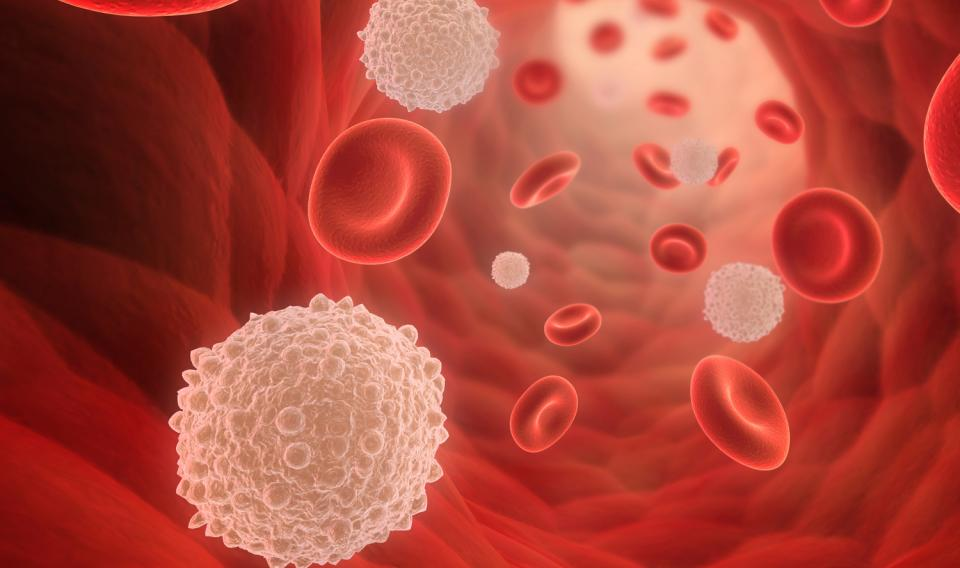
\includegraphics[width=3cm]{bloodcells.jpg}\\
	%			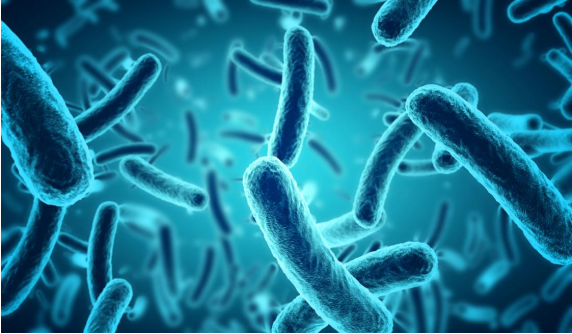
\includegraphics[width=3cm]{bacteria.png}\\			
	%			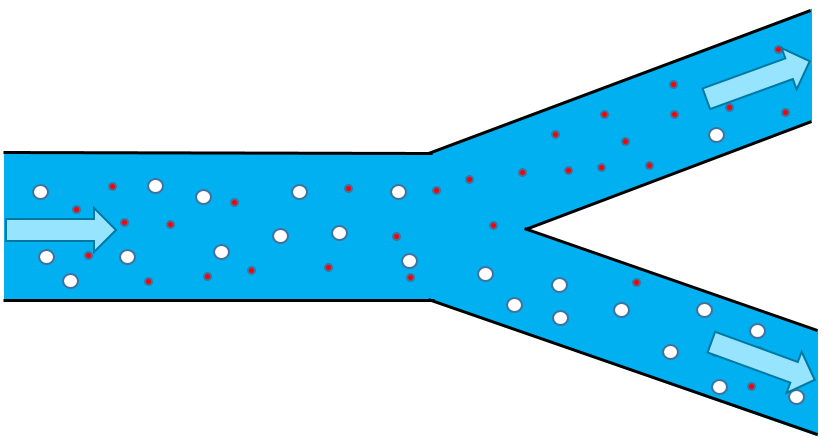
\includegraphics[width=3cm]{Microfilter.png}\\
	%			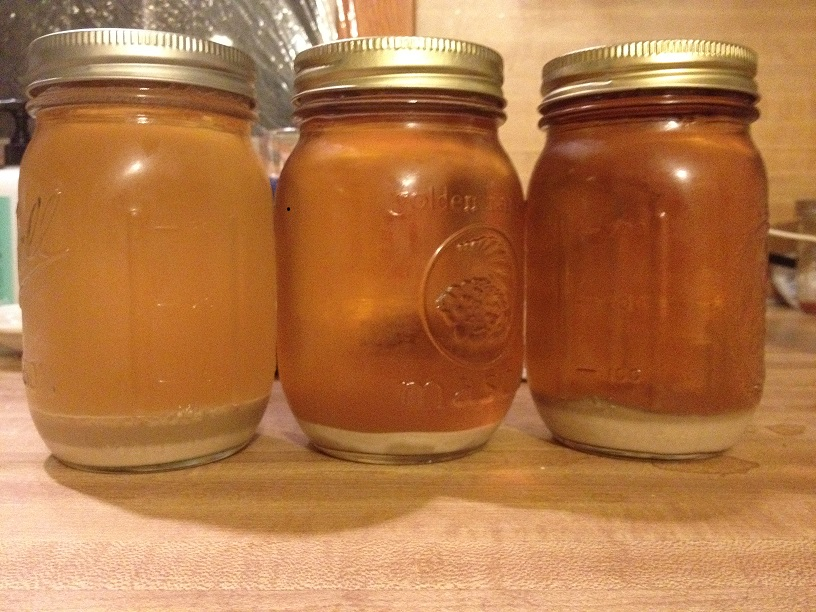
\includegraphics[width=3cm]{beer.png}
	%		\end{figure}
	%	\end{columns}
\end{frame}



\begin{frame}
	\frametitle{Newton Krylov Result 2D}
	\vspace{0.3cm}
	Overall Cost: $\mathcal J = \frac{1}{2}\norm{\rho- \widehat{\rho}}_{L_2(\Sigma)}^2 + \frac{\beta}{2} \norm{\vec{w}}_{L_2(\Sigma)}^2$, $\mathcal J_{\vec{w} = \vec 0} = 0.0209$, $\mathcal J_{opt} = 0.0026$.
	\begin{figure}
		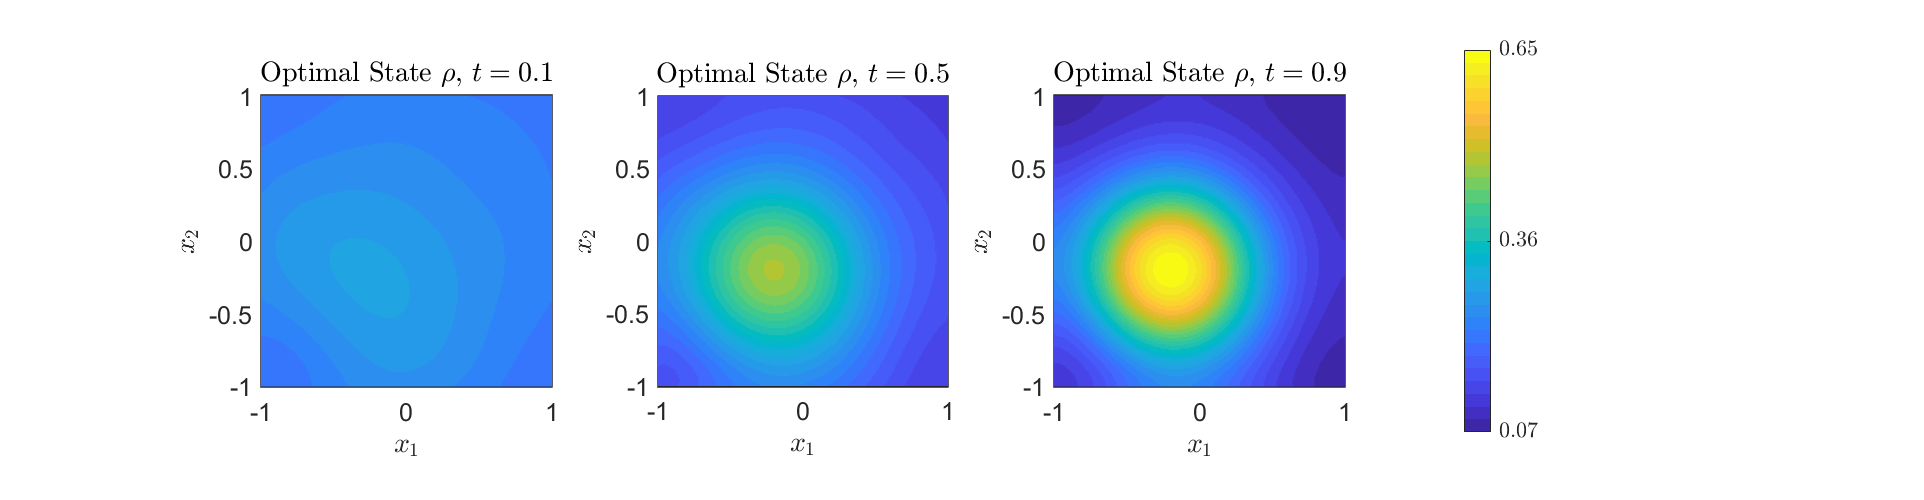
\includegraphics[width=13.5cm]{FCNkn1.png}
		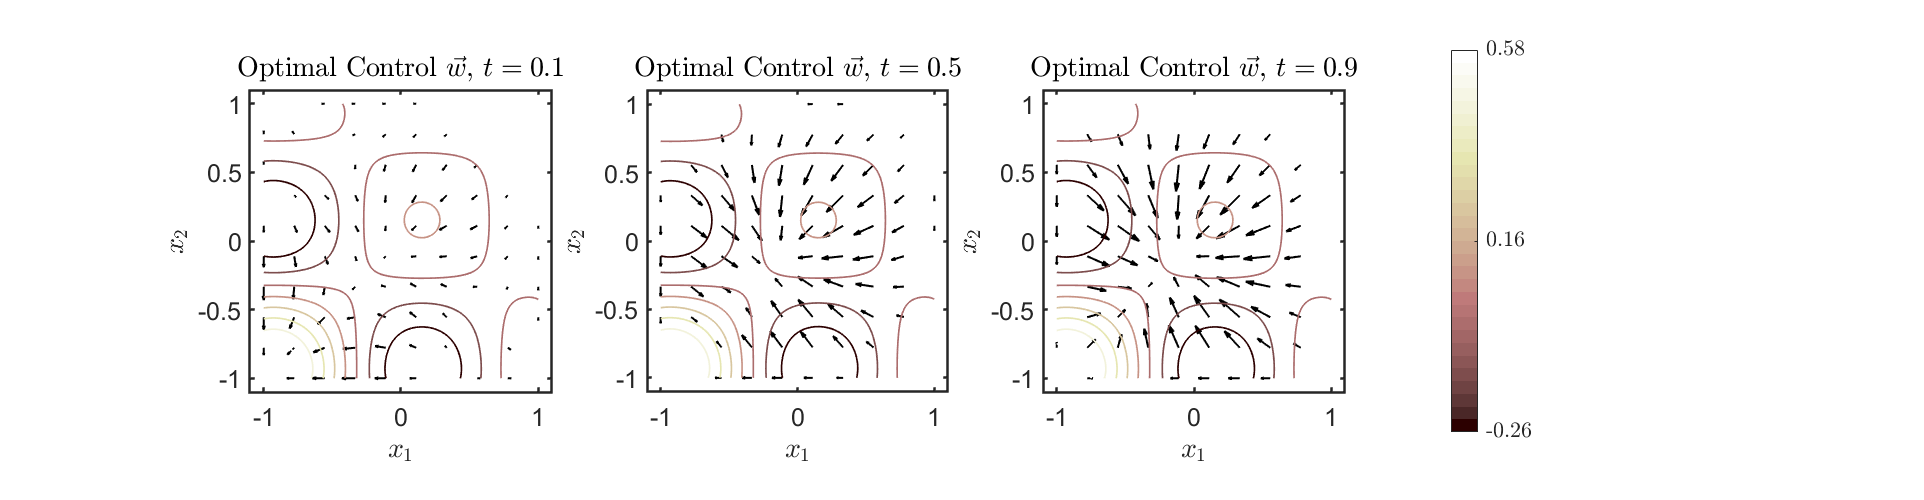
\includegraphics[width=13.5cm]{FCNkn1c.png}
	\end{figure}
\end{frame}


\begin{frame}
	\frametitle{Newton Krylov Result 3D}
	\vspace{0.3cm}
	Overall Cost: $\mathcal J = \frac{1}{2}\norm{\rho- \widehat{\rho}}_{L_2(\Sigma)}^2 + \frac{\beta}{2} \norm{\vec{w}}_{L_2(\Sigma)}^2$, $\mathcal J_{\vec{w} = \vec 0} = 0.0477$, $\mathcal J_{opt} = 0.0059$.
	\vspace{0.3cm}
	\begin{figure}
		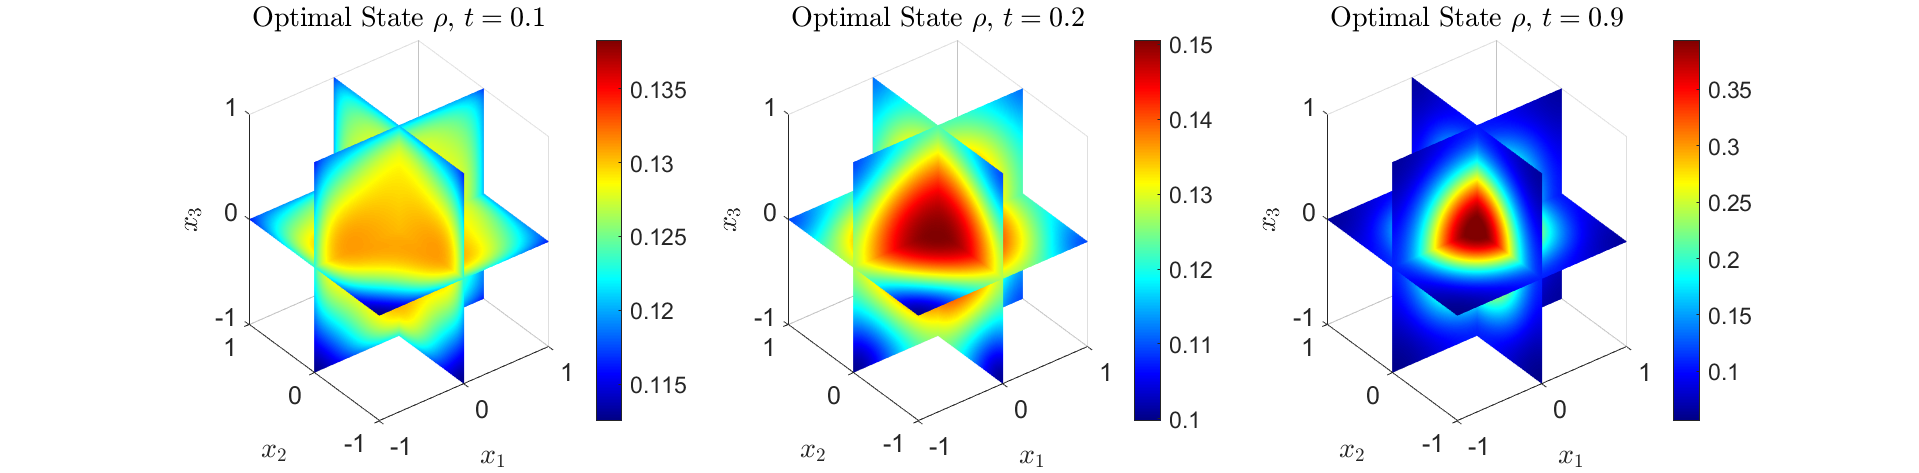
\includegraphics[width=15cm]{rhokn1.png}
	\end{figure}
	
\end{frame}
\begin{frame}
	\frametitle{Newton Krylov Result 3D}
	\vspace{0.3cm}
	Overall Cost: $\mathcal J = \frac{1}{2}\norm{\rho- \widehat{\rho}}_{L_2(\Sigma)}^2 + \frac{\beta}{2} \norm{\vec{w}}_{L_2(\Sigma)}^2$, $\mathcal J_{\vec{w} = \vec 0} = 0.0477$, $\mathcal J_{opt} = 0.0059$.
	\vspace{0.3cm}
	\begin{figure}
		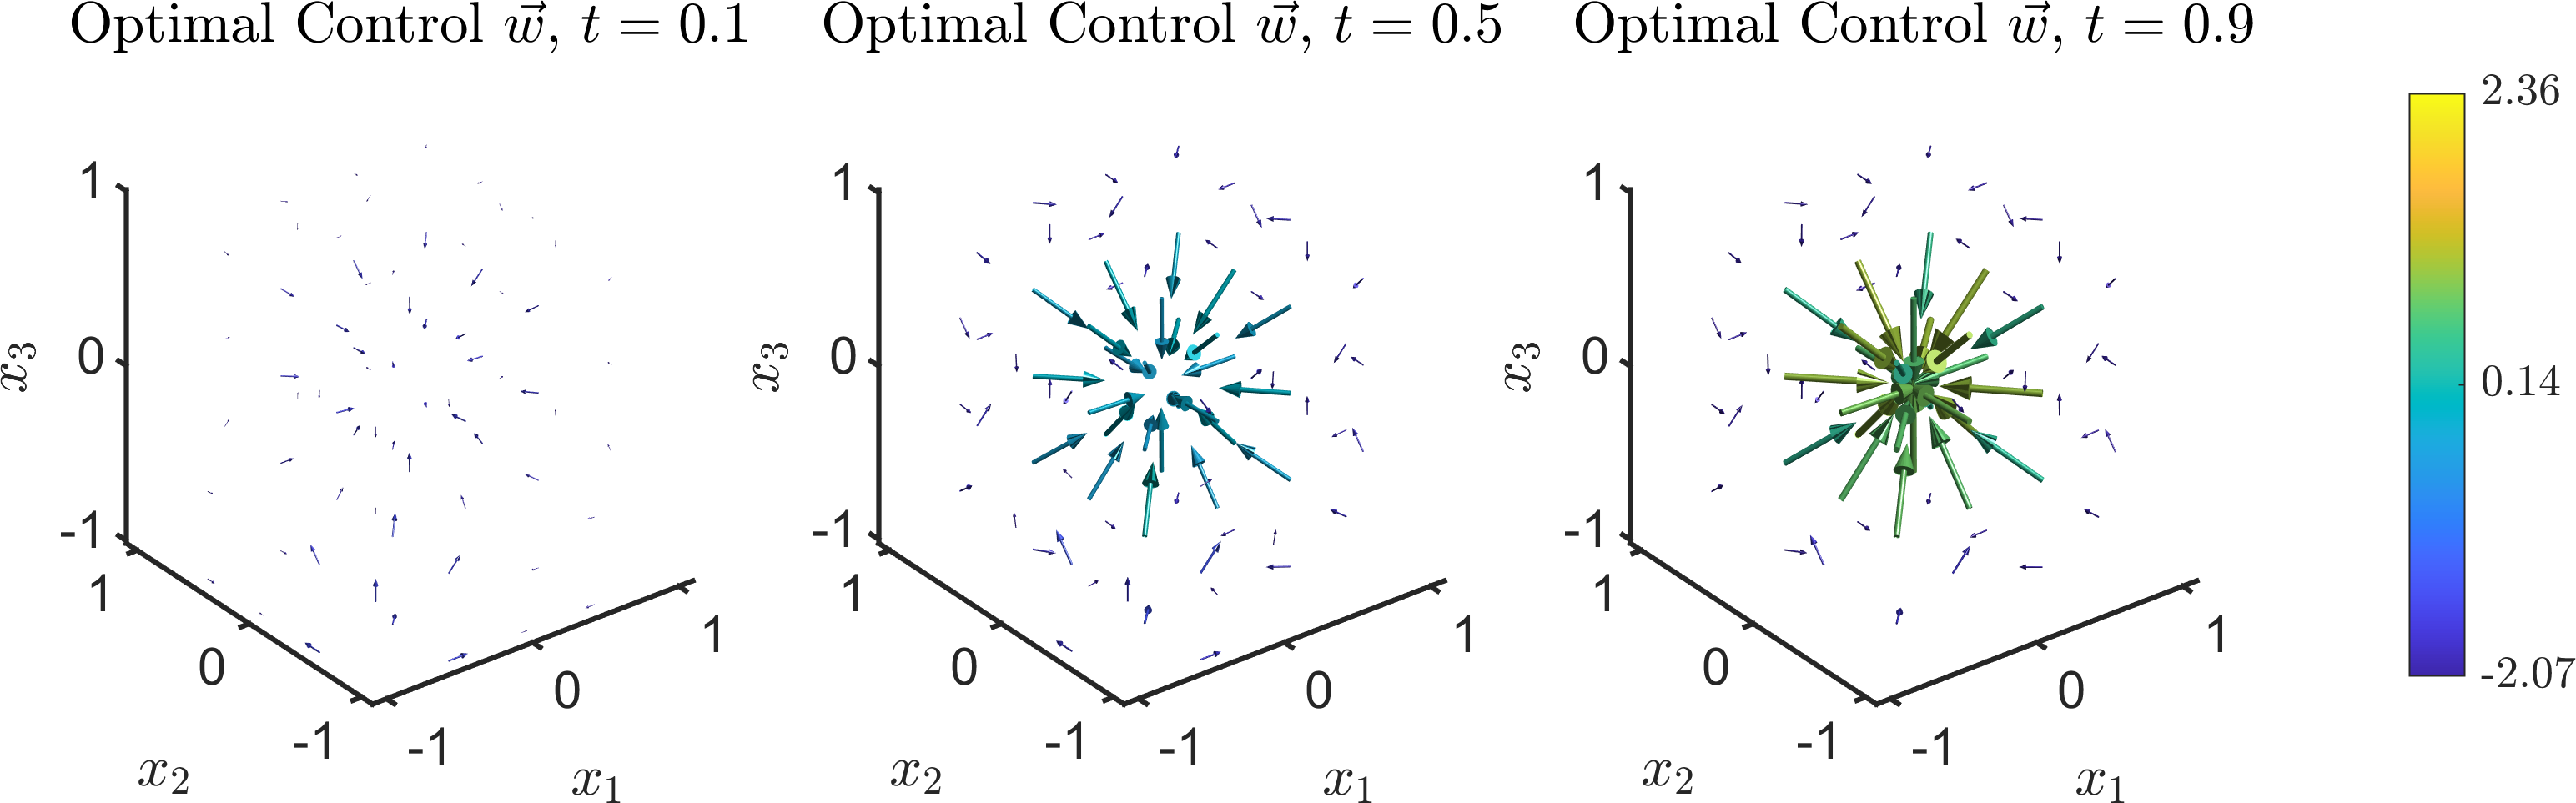
\includegraphics[width=13cm]{Controlkn1.png}
	\end{figure}
	
\end{frame}

\begin{frame}
	\frametitle{Next steps}
	\textbf{Industrial partners of the PhD}
	\begin{columns}
		\column{0.5 \linewidth}
		\begin{figure}
			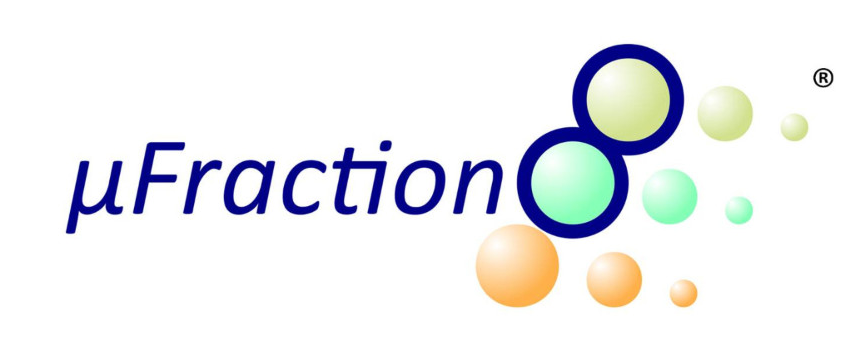
\includegraphics[width=5cm]{ufraction8.png}
			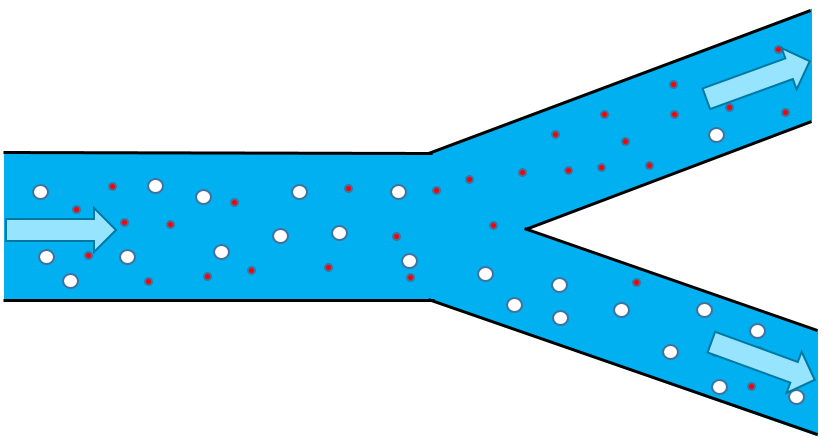
\includegraphics[width=5cm]{Microfilter.png}
			%\caption{Nanofiltration Device}
		\end{figure}
		
		\column{0.5 \linewidth}
		\begin{figure}
			
\includegraphics[width=3cm]{west.png}\\
			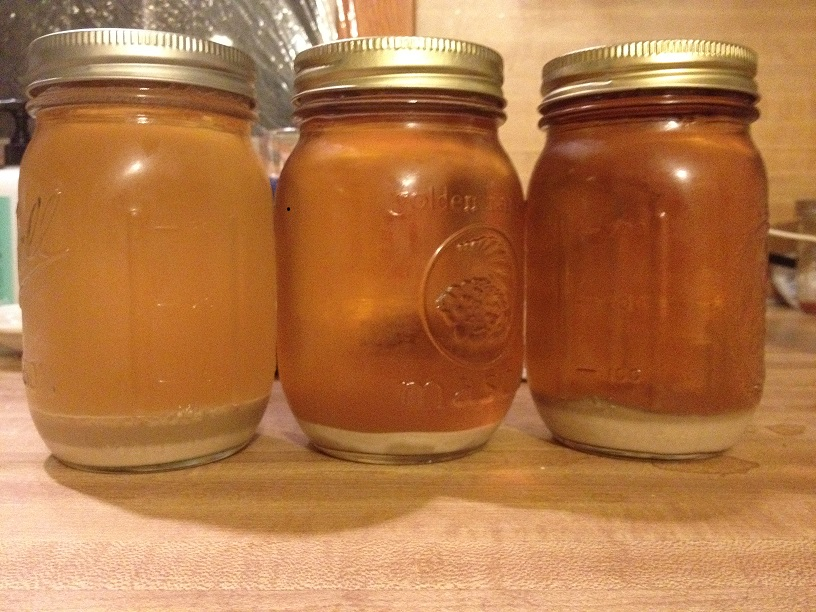
\includegraphics[width=3.5cm]{beer.png}
			%\caption{Yeast Sedimentation in Beer}
		\end{figure}
	\end{columns}
\end{frame}

\begin{frame}
	\frametitle{Summary}
	Up to now:
	\begin{itemize}
		\item Developed a numerical framework for solving PDE-constrained optimization problems.
	\end{itemize}
	Current:
	\begin{itemize}
		\item More complex domains.
		\item Extended models.
		\item Different boundary conditions.
	\end{itemize}
	Up next:
	\begin{itemize}
		\item Application of the Newton-Krylov Algorithm to more complex domains.
		\item Application of the method to other extended models.
		\item Application of the numerical framework to industrial processes.
	\end{itemize}
	
\end{frame}

\appendix
\begin{frame}
	\printbibliography
	
\end{frame}

\begin{frame}
	\frametitle{2D Results Table}
	\begin{table}
\centering
\begin{tabular}{ | c | c || c | c | c | c | c ||}
\hline
\multicolumn{2}{|c||}{}& $\beta = 10^{-5}$ & $\beta = 10^{-3}$ & $\beta = 10^{-1}$ & $\beta = 10^{1}$ & $\beta = 10^{3}$  \\
\hline
\hline
\multirow{2}{*}{$\kappa= \numprint{0}$}  & $\mathcal{J}_{uc}$ & $\numprint{2.67e-2}$ & $\numprint{2.67e-2}$ & $\numprint{2.67e-2}$ & $\numprint{2.67e-2}$ & $\numprint{2.67e-2}$\\
 & $\mathcal{J}_c$ & $\numprint{8.23e-5}$ & $\numprint{3.87e-3}$ & $\numprint{2.50e-2}$ & $\numprint{2.67e-2}$ & $\numprint{2.67e-2}$\\
\hline
\multirow{2}{*}{$\kappa= \numprint{1}$}  & $\mathcal{J}_{uc}$ & $\numprint{3.29e-2}$ & $\numprint{3.29e-2}$ & $\numprint{3.29e-2}$ & $\numprint{3.29e-2}$ & $\numprint{3.29e-2}$\\
 & $\mathcal{J}_c$ & $\numprint{1.16e-4}$ & $\numprint{5.44e-3}$ & $\numprint{3.13e-2}$ & $\numprint{3.29e-2}$ & $\numprint{3.29e-2}$\\
\hline
\multirow{2}{*}{$\kappa= \numprint{-1}$}  & $\mathcal{J}_{uc}$ & $\numprint{2.09e-2}$ & $\numprint{2.09e-2}$ & $\numprint{2.09e-2}$ & $\numprint{2.09e-2}$ & $\numprint{2.09e-2}$\\
 & $\mathcal{J}_c$ & $\numprint{5.71e-5}$ & $\numprint{2.63e-3}$ & $\numprint{1.92e-2}$ & $\numprint{2.09e-2}$ & $\numprint{2.09e-2}$\\
\hline
\end{tabular}
\caption{Flow Control No-Flux Problem: Cost when $\vec{w}=\vec{0}$ and optimal control cost for a range of $\kappa$, $\beta$. Note that for $\beta = 10$, the cost functionals differ by $10^{-5}$, while for $\beta = 10^3$ they differ by $10^{-7}$ (++ two in the wrong direction ++).}
\label{TabFCN}
\end{table}
\end{frame}

\begin{frame}
	\frametitle{Optimization for DDFT}
	\framesubtitle{A more general DDFT model}
	\begin{align*}
		&\min_{\rho,\vec{w}} \quad \frac{1}{2}\norm{\rho- \widehat{\rho}}_{L_2(\Sigma)}^2 + \frac{\beta}{2} \norm{ {\vec{w}}}_{L_2(\Sigma)}^2\\
		\\
		&\text{subject to:}
		\\
		& \ \partial_t \rho = \nabla \cdot \left( \rho \nabla \frac{\delta \textcolor{RoyalBlue}{ \mathcal F [\rho]} }{\delta \rho} - \rho  {\vec{w}}\right):= - \nabla \cdot \vec j \qquad \ \ { \text{in    } \Sigma}\qquad\qquad\qquad\qquad\\
		&\textcolor{RoyalBlue}{ \mathcal F [\rho]=  \mathcal F_{id}[\rho] + \mathcal F_{ext}[\rho] +  \mathcal F_{int}[\rho] + \int_\Omega \rho \left(-1 -\ln(1 - a\rho) + \frac{1}{1-a\rho}  \right)d \vec x} \\
		\\
		&{\text{BC } \text{and IC:}}\\
		&\vec j \cdot \vec n = 0 \quad \ \qquad \quad \qquad \qquad\qquad\qquad\qquad\qquad \text{on   } \partial \Sigma   \qquad\qquad\qquad\qquad\qquad \qquad \qquad\qquad \qquad \qquad\\
		&{\rho(0,\vec{x}) = \rho_0(\vec{x})} 
	\end{align*}
\end{frame}
\begin{frame}
	\frametitle{Deriving optimality conditions}
	\textbf{Deriving (first-order) optimality conditions}\\
	Define the Lagrangian $\mathcal{L}(\rho, \vec{w}, q)$:
	\begin{align*}
		\mathcal{L}(\rho, \vec{w},q)&= \frac{1}{2}\norm{\rho- \widehat{\rho}}_{L_2(\Sigma)}^2 + \frac{\beta}{2} \norm{\vec{w}}_{L_2(\Sigma)}^2\\
		&+ \int_\Sigma q\bigg( \partial_t \rho - \nabla^2 \rho + \nabla \cdot (\rho \vec{w})
			- \nabla \cdot\int_\Omega \rho(\vec{x}) \rho(\vec{x}\hspace{0.2em}') \nabla V_2(|\vec{x}-\vec{x}\hspace{0.2em}'|)d\vec{x}\hspace{0.2em}'   \bigg) d\vec{x} dt\\
		&+ \int_{\partial \Sigma} q  \bigg(\frac{\partial \rho}{\partial n} - \rho \vec{w} \cdot \vec{n} +  \int_\Omega \rho(\vec{x}) \rho(\vec{x}\hspace{0.2em}')  \frac{ \partial  V_2}{\partial n}(|\vec{x}-\vec{x}\hspace{0.2em}'|)d\vec{x}\hspace{0.2em}' \textcolor{gray}{\bigg)} d\vec{x} dt\\
	\end{align*}
	1. Take derivatives of $\mathcal{L}(\rho, \vec{w}, q)$ with respect to $\rho$, $\vec{w}$ and $q$. \\
	2. Set derivatives to zero to find stationary points. \\
\end{frame}



\begin{frame}
	\frametitle{Figure References}   
	\begin{thebibliography}{10}    
		
		\bibitem{F3}
		ufraction8 Logo. Digital Image. \newblock{ \em www.ufraction8.}
		\url{ufraction8.com}
		
		\bibitem{F4}
		WEST Logo. Digital Image. \newblock{\em WEST Brewery} \url{www.westbeer.com}
	\end{thebibliography}	
\end{frame}
\begin{frame}
	\frametitle{Some References}    
	\cite{Us2020} and
	\cite{Author1990}
	
\end{frame}

\end{document}